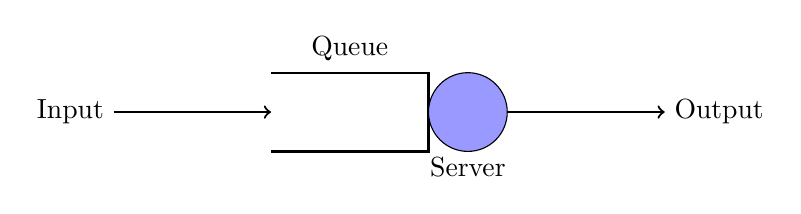
\begin{tikzpicture}
    % Draw the queue block (left-open rectangle)
    \draw[thick] (0, 0.5) -- (2, 0.5) -- (2, -0.5) -- (0, -0.5);
    \node at (1, 0.8) {Queue};

    % Draw the input arrow
    \draw[->, thick] (-2, 0) -- (0, 0);
    \node[left] at (-2, 0) {Input};

    % Draw the server (circle)
    \filldraw[fill=blue!40, draw=black] (2.5, 0) circle (0.5);
    \node at (2.5, -0.7) {Server};

    % Draw the output arrow
    \draw[->, thick] (3, 0) -- (5, 0);
    \node[right] at (5, 0) {Output};
\end{tikzpicture}